\subsection{Traffic Demand Per Subscriber}\label{subsec:behavior}

\begin{figure}[t]
\begin{minipage}{1\linewidth}
\centering
%
\begin{subfigure}[b]{1\linewidth}
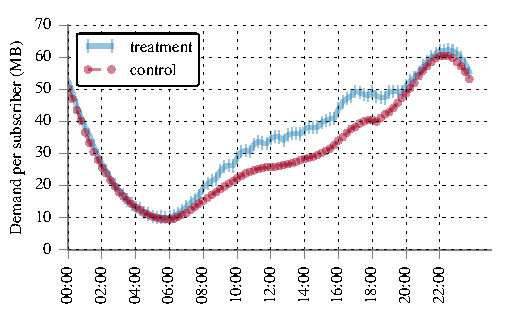
\includegraphics[width=\linewidth]{figures/weekday_demand_mean.pdf}
               \caption{Weekday traffic demand\label{fig:weekday-daily-usage}}
\end{subfigure}
%
\begin{subfigure}[b]{1\linewidth}
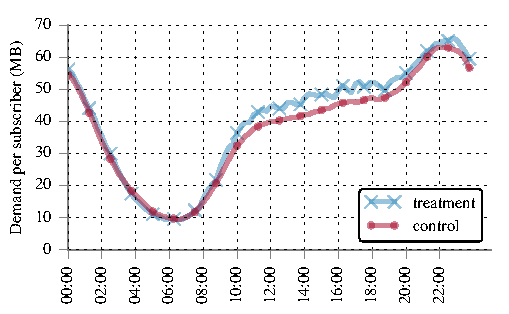
\includegraphics[width=\linewidth]{figures/weekend_demand_mean.pdf}
               \caption{Weekend traffic demand\label{fig:weekend-daily-usage}}
\end{subfigure}
%
\end{minipage}
\caption{Average subscriber demand (bytes every 15-minutes)}
\label{fig:traffic-demand-timeseries}
\end{figure}

Figure \ref{fig:traffic-demand-timeseries} shows the downlink traffic demand (bytes)
of an average subscriber over a 15-minute measurement period in a week.
We observe that subscriber behavior differs
significantly on weekdays and weekends. On weekdays, traffic demand 
increases monotonically from morning until prime-time in the evening. On 
weekends, there is a sharp rise in demand in the early morning period. Then, the
demand plateaus until the next sharp rise during the evening prime-time hours.
Previous reports indicate that the aggregate traffic volume for US fixed access
link providers usually troughs during mid-afternoon hours (between 2:00 PM -- 6:00 PM)
~\cite{sandvine20141h}. We do not observe such a trough in the subscriber 
demand in our dataset.

\begin{figure}[t]
\begin{minipage}{1\linewidth}
\centering
%
%\begin{subfigure}[b]{.33\linewidth}
%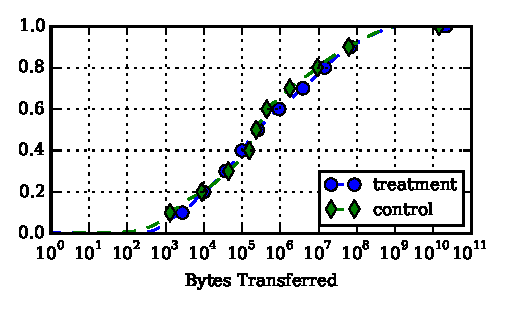
\includegraphics[width=\linewidth]{figures/cdf-all-bytes.pdf}
%                \caption{Overall traffic demand for all subscribers at all times\label{fig:CDF-data-rate}}
%\end{subfigure}
% maybe should be mean per day?
%
\begin{subfigure}[b]{1\linewidth}
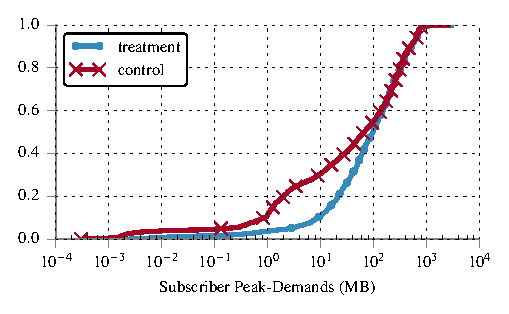
\includegraphics[width=\linewidth]{figures/cdf_peak_demand-overall.pdf}
               \caption{Peak (95\%) traffic demand per subscriber\label{fig:CDF-data-rate-perc95}}
\end{subfigure}
%
% COMMENT OUT IF TAKING TOO MUCH SPACE
\begin{subfigure}[b]{1\linewidth}
 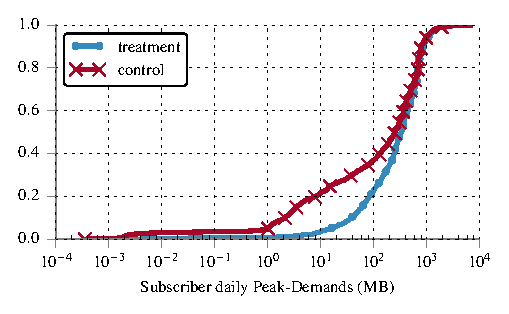
\includegraphics[width=\linewidth]{figures/cdf_peak_demand-daily.pdf}
                \caption{Peak (95\%) traffic demand per subscriber\label{fig:CDF-data-rate-daily-perc95}}
 \end{subfigure}
%
\end{minipage}
\caption{Traffic demand (bytes every 15-minutes) for \control{} and \treatment{}\label{fig:traffic-demand-cdf}}
\end{figure}

Figure \ref{fig:CDF-data-rate-perc95} shows the distribution of the
the 95th percentile of downlink traffic demand (bytes transferred)
in the \treatment{} and \control{} set
over the three month measurement period. The meaximum peak
demand achieved by subscribers in the \control{} and \treatment{}
groups was 2.67 GB and 3.0 GB respectively. The average peak traffic
demand was 169.8 MB for \control{} and 186.6 MB for \treatment{}.
Given the 105 Mbps service tier, this means that users rarely utilize
their links (average utilization of a 105 Mbps link even at the
overall 95th percentile was 1.43\% for \control{} and 1.5\% for \treatment{})

The median peak demand was 66.7 MB for the lower tier, and
98.4 MB for thj. We expected the largest difference
in demands would be in the subscribers who have the heaviest demand in
both groups, as they are the ones who utilize most of the link.
But unexpectedly, the lowest demanding 50\% of the subscribers have
a substantial difference in peak demands. The low demanding subscribers
of the \treatment{} group have a higher demand than the lowest demanding 50\% of
\control{}. We confirm that the both groups have similar median demands over each day. However
the daily peak demand is higher for the lowest demanding subscribers in
 \treatment{}, as compared to the lowest demanding subscribers in \control{}.

%\begin{figure}[t]
%\centering
%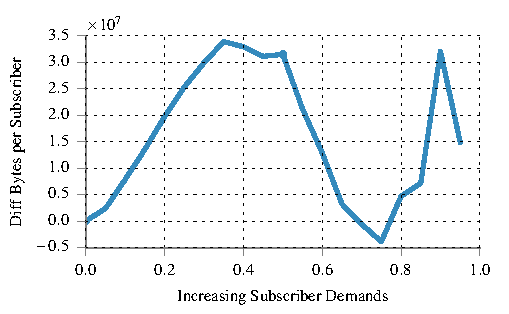
\includegraphics[width=\linewidth]{figures/diff_perc95_bytes_subsc-overall.pdf}
%               \caption{Difference between \treatment{} and \control{}
%               in peak (95\%) traffic demand\label{fig:diff-perc95}}
%\end{figure}

 
\begin{figure}[t]
\begin{minipage}{1\linewidth}
\centering
%
\begin{subfigure}[b]{.99\linewidth}
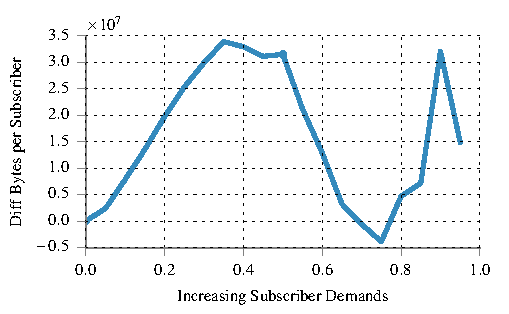
\includegraphics[width=\linewidth]{figures/diff_perc95_bytes_subsc-overall.pdf}
               \caption{Overall peak (95\%) per subscriber\label{fig:diff-peak-overall}}
\end{subfigure}
% 
% COMMENT OUT IF TAKING TOO MUCH SPACE
\begin{subfigure}[b]{.99\linewidth}
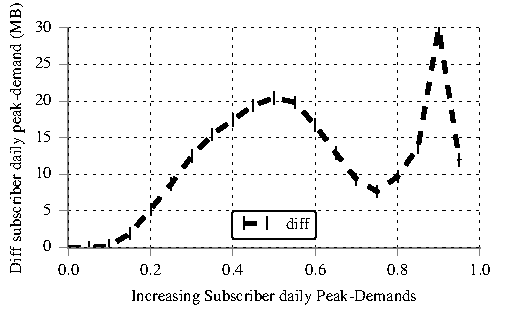
\includegraphics[width=\linewidth]{figures/diff_perc95_bytes_subsc-daily-overall.pdf}
                \caption{Daily peak (95\%) per subscriber\label{fig:diff-peak-daily}}
\end{subfigure}
%
\end{minipage}
  \caption{Difference between peak-demands of subscribers from \treatment{} and
  \control{} groups. Subscribers were considered at every 5\% in each group.
  \label{fig:diff-peak}}
\end{figure}


We plot the distribution of the difference in peak subscriber demands for
the lowest to highest demanding subscribers in both groups (Figure~\ref{fig:diff-peak}).
We also plot the distributions on log scale along with the difference.
As both groups had a different number of subscribers, we sort their peak demands
and consider values at every 5th percentile to calculate the difference.
From figure ~\ref{fig:diff-peak-overall}, we see that the overall peak demand for the
lowest demanding 70\% of the households of the \treatment{} group is higher than
the peak demand of the lowest demanding bottom-most
70\% of the \control{} group. These subscribers have a peak demand less than 200 MB.
For 20\% of the subscribers compared, the peak demand of the \treatment group is 30 MB
higher than the \control group. These consist of subscribers in the lower tier
control group with a peak demand between 10 -- 70 MB, and subscribers in the higher
tier with peak demand between 40 -- 100 MB.

Under 15\% of subscribers in the \treatment{} group have peak demands more than 200 MB
but less than 400 MB. p
eak demands similar, or lower than the equivalent 15\% of subscribers in the \control{}
group, that has a lower capacity. The highest demanding subscribers in the \treatment{}
(beyond 800 MB peak demand) have demands 15 -- 30 MB more than the equivalent 15\% of 
the \control{} group. For the upstream, the \treatment{} group consistently has
a 2 MB higher peak traffic demand every 15 minutes as compared to the \control{} group
(except for the top 10\% users in the \treatment{} set who had a higher peak).

%\begin{figure}[t]
%\centering
%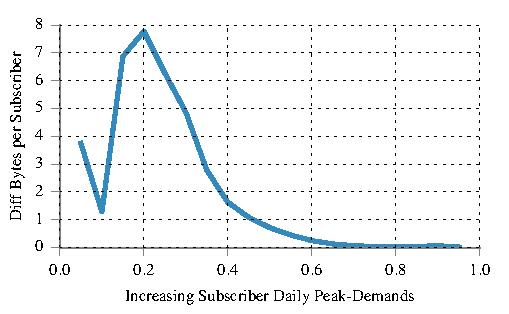
\includegraphics[width=\linewidth]{figures/diff_perc95_bytes_subsc-daily-normalized.pdf}
%               \caption{Ratio of the difference between \treatment{} and \control{}
%               in the daily peak traffic demand to the daily peak of the \control\label{fig:daily-ratio-perc95}}
%\end{figure}

On investigating further, we observed that a similar percentage of 
subscribers with low peak demand in \control{} had a higher peak demand in \treatment{} every
day (Figure~\ref{fig:diff-peak-daily}).
40\% of the subscribers with lowest daily peak demands in the \treatment{} still
had more than double the traffic demand of the equivalent 40\% in the \control{} group.
%(see Figure~\ref{fig:daily-ratio-perc95}).

There could be many reasons for this increase in demand for subscribers that
have lower peak demands. One reason could be short term web activities (such as short videos,
web browsing) that have a slightly higher traffic demand. Such an increase in demand would then
be apparent during hours when users pursue such activities. Another reason could be
an increase in background traffic (such as software updates). Although studying the applications 
responsible for such behavioral changes in traffic demand is not in the scope of our
work, an interesting question that arises is: when does the demand increase the most 
throughout a day?